\section{Optimization} \label{sec:opt}
\subsection{Equivalence Class Consolidation}
To minimize the amount of temporal verification overhead, we want to find some symmetry in the 
existing exploration algorithm so that we could reduce the exploration space even further.

In the original NetDice exploration algorithm, multiple network states were merged into an Equivalence 
Class based on its cold edges (edges whose failure won't change the convergent path(s)).
In other words, network states within the same Equivalence Class will have the same convergent path(s).

However, we observe that each of those Equivalence Classes are not \textit{unique}: while network states within 
the same equivalence class shares a convergent path(s), \textbf{multiple equivalence classes could also 
share the exact same convergent path(s)}, as shown in $\mathcal{E}_2$ and $\mathcal{E}_3$ in Fig. \ref{fig:tree}.

Since we define latency distribution to marginalize over all factors other than the path, we could 
effectively \textit{consolidate} these equivalence classes into one big equivalence class and do temporal 
verification once.

We implemented this idea by doing memoization on the temporal probability of a given convergent path(s).
We will only do temporal probability computation once, when we first iterate over an equivalence class that 
has a certain convergent path(s), and we cached the result should another equivalence class with the same 
convergent path(s) emerged.

\subsection{Path Memoization}
After consolidating many equivalence classes that shares the same convergent path(s), we are left with fewer, 
bigger, but unique equivalence classes.
As significant as it is, we could reduce the computation cost further by drawing connections between these 
unique equivalence classes.

In a network with a load-balancing protocol, the convergent state of the data plane might forward a packet 
through multiple possible paths.
In the context of our framework, we say that an equivalence class might have more than one convergent paths.
Nevertheless, we note that two equivalence classes with different convergent paths might not be two 
independent subset.
In other words, \textbf{multiple equivalence classes could share a subset of individual path}.

Since the way we compute convergent path(s) temporal probability is by calculating the weighted average of 
individual path temporal probability, we could reduce the amount of convolution we will need to do by doing further memoization 
on the temporal probability of a given path.
If we were to compute the temporal probability of an equivalence class with previously cached individual 
path, we only need to calculate the weights that corresponds to the load balancing protocol without 
doing any convolution.

In our running example, we could see that in Fig. \ref{fig:tree}, $\mathcal{E}_2$ and $\mathcal{E}_4$ share 
an identical path, $SDET$.
We could therefore memoize $cdf(\mathcal{L}_{SDET}, t)$ when we explore $\mathcal{E}_2$ and query the 
cached result when we explore $\mathcal{E}_4$.

With this optimization, we will do a chain convolution by the amount of path available in the network between 
the source and destination (which is 3 in the case of our running example in Fig. \ref{fig:ex}: $SAT$, $SBCT$, 
and $SDET$).

% \subsection{Convolution Grouping}
% Aside from optimizing the \textit{amount} of paths we need to do convolution on, we could also do some 
% optimization on the \textit{convolution operation itself}. 

% \begin{figure}[h]
%     \centering
%     % 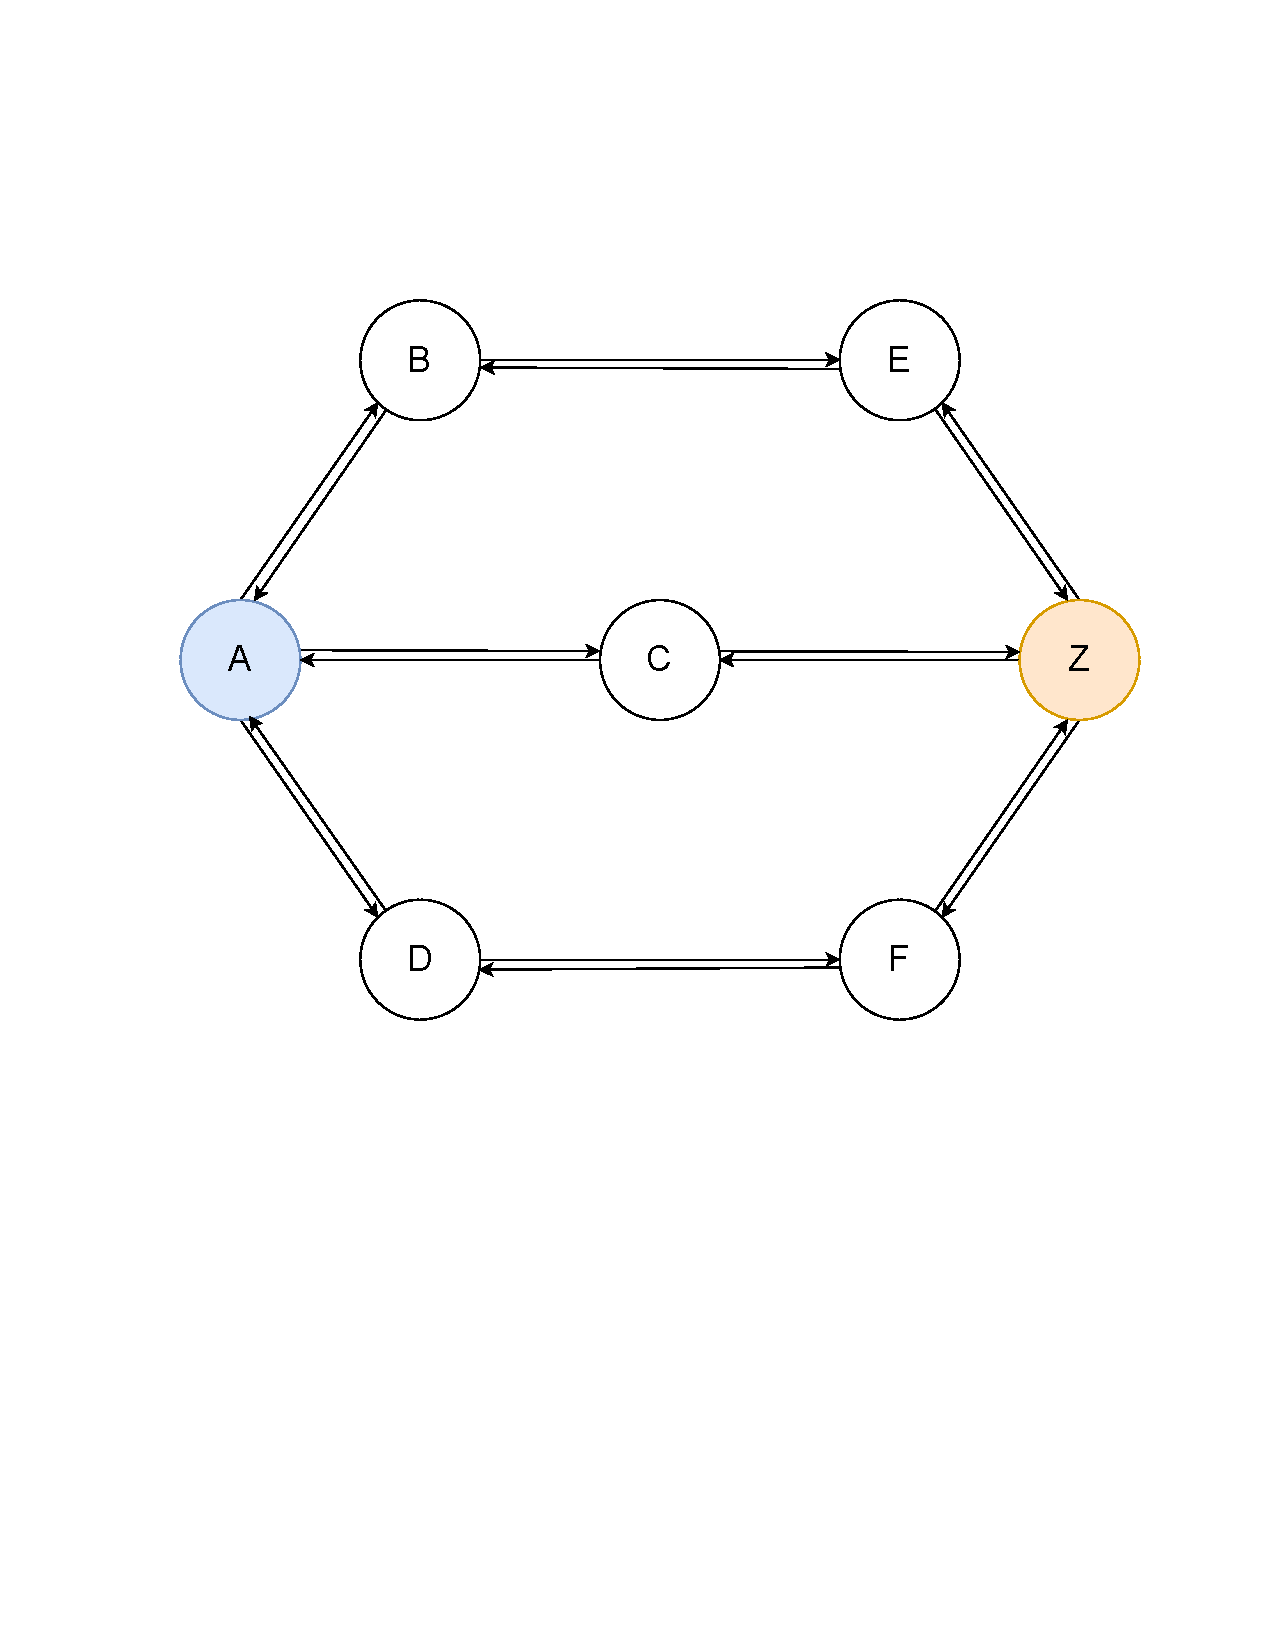
\includegraphics[width=0.4\textwidth, trim=0cm 11cm 0cm 5cm]{ex.pdf}
%     \includegraphics[width=\columnwidth]{../tikz/group}
%     % 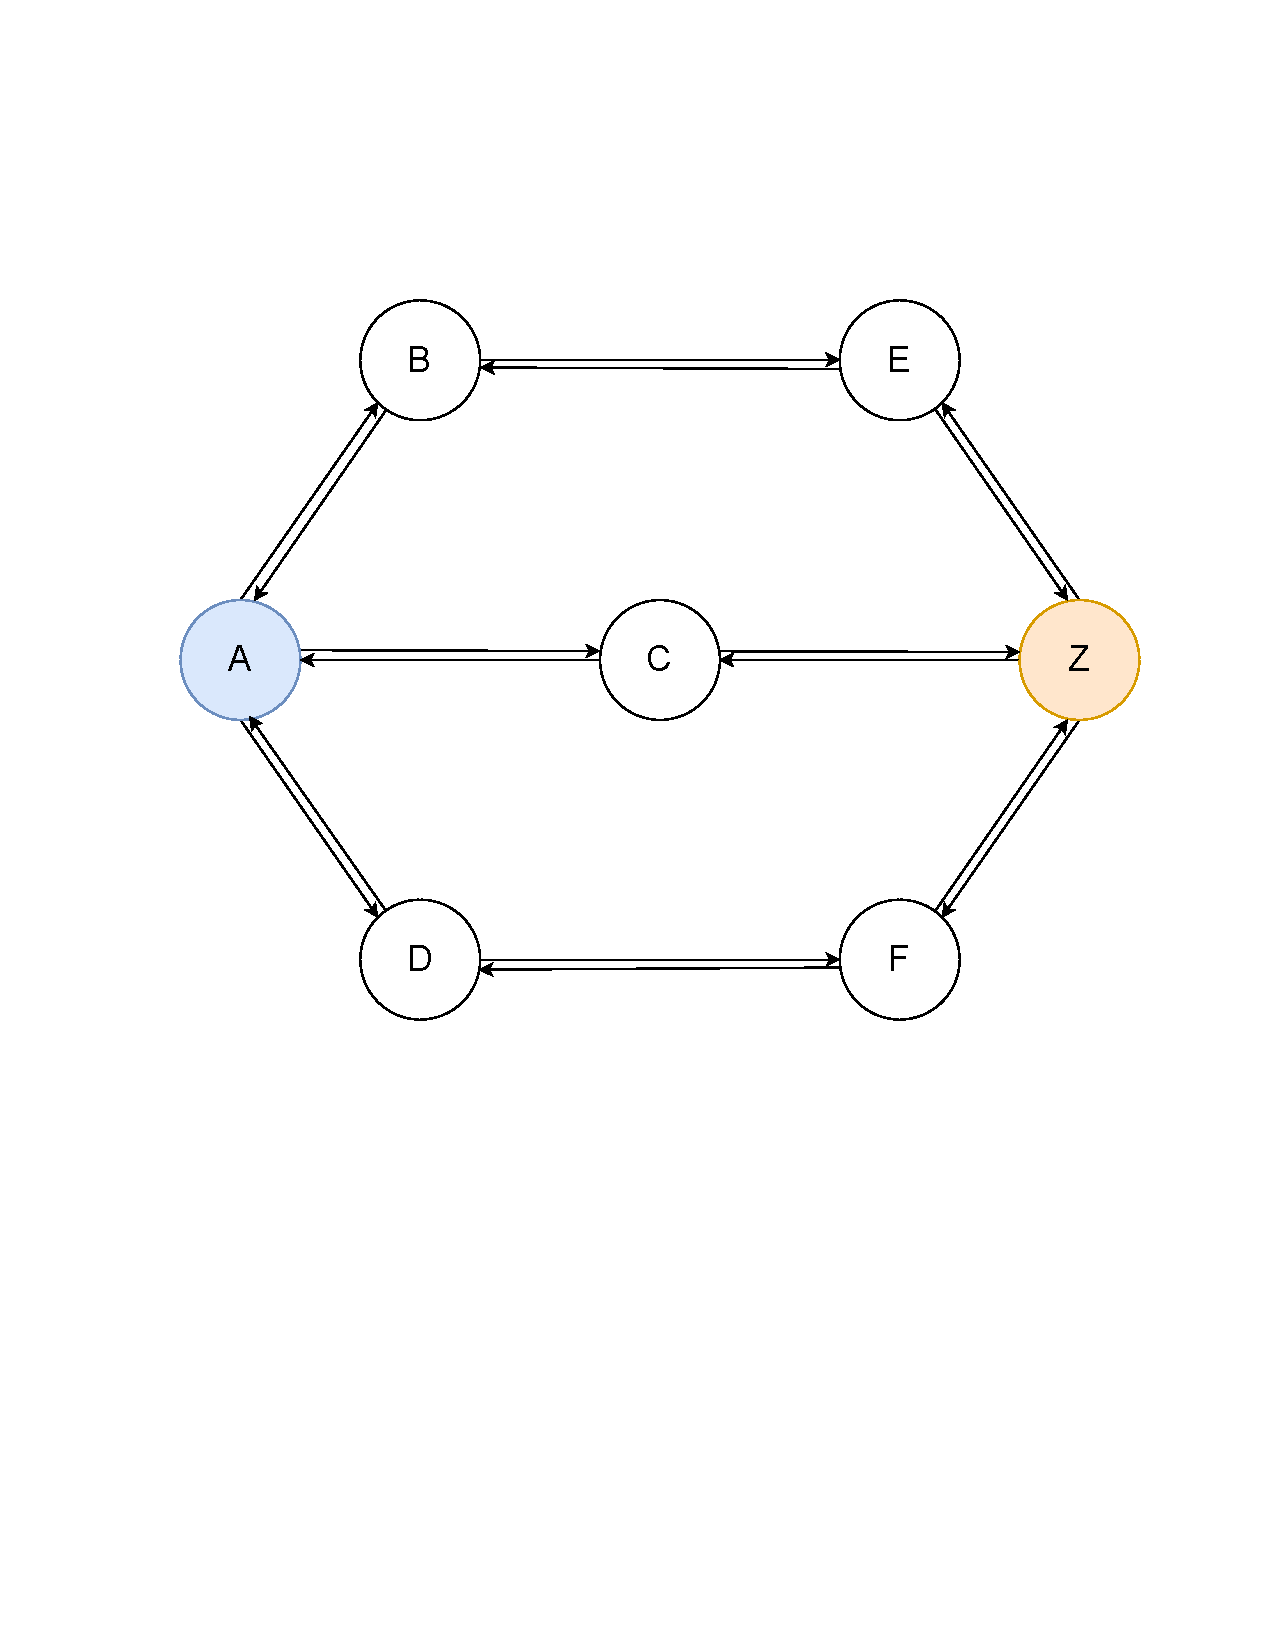
\includegraphics{ex.eps}
%     \caption{One example of a convolution tree to get $\mathcal{L}_{ABEZ}$ with optimized grouping,
%     we want to start introducing numerical convolution as late as possible}
%     \label{fig:grouping}
% \end{figure}

% While the use of numerical technique to do convolution enabled us to use arbitrary probability distribution 
% in our framework, it comes with two noticeable disadvantages.

% The first is \textit{error}: numerical method is fundamentally an approximation technique that always 
% comes with some error. 
% While DIRECT algorithm comes with an error-bound guarantee, it is not zero and could expand if we do 
% chain convolution.

% The second is \textit{runtime performance}: even with the input ordering constraints we laid out on the 
% previous subsection, DIRECT is still generally slower than analytical convolution.
% This is expected, since a closed form solution of a convolution tipically boils the operation down into 
% a few arithmetic calculation, rather than complex operation like integration.
% Due to these factors, we feel the need to \textbf{prioritize analytical convolution} in the calculation of 
% path latency distribution.

% We did this by \textit{grouping} subsets of the path components with the same probability distribution 
% type (e.g. exponential, normal, etc.). 
% We then analytically convolve the distribution within that subset and only numerically convolve the 
% returned distribution, which will be fewer in quantity, thus enabling smaller error and faster performance.

% In our running example, in the chain convolution process to get $\mathcal{L}_{ABEZ}$, we will analytically
% convolve $l_p(AB)$, $l_q(AB)$, $l_p(BE)$, $l_q(BE)$, and $l_p(EZ)$ since they are of the same type (gamma) 
% and then numerically convolve the resulting distribution with $l_q(EZ)$.
% Fig. \ref{fig:grouping} illustrates how the chain convolution process will be broken down.

% \textbf{First}, we do the functional verification with $G_t$ similar to what NetDice 
% \cite{netdice} have done. 
% In addition, we also collect additional information from each state (e.g. convergent 
% paths) to be used in the temporal verification step. 

% \textbf{Second}, we compute the total path latency distribution from the convergent path(s) in each 
% state with $G_l$.
% This is done by convolving over the latency distribution of each component in the path. 
% Since not all convolutions can be calculated analytically, we implemented a numerical convolution 
% method via mixture distribution, DIRECT \cite{direct}, which is able to convolve two 
% distribution with a KL divergence error bound.
% Multiple states can share the same convergent path(s), so \textit{only a fraction of the states need to be 
% explored}.

% \textbf{Third}, we calculate the probability of a given temporal property being true in that state. 
% For example, given a \textit{bounded reachability property} (probability of whether a packet can 
% traverse from a source to destination below some time unit $T$), we can compute its probability by 
% integrating the PDF from $0$ to $T$. 
% We then combine all of the \textit{temporal} and \textit{functional} probability in each state to 
% get the final probability: the probability of \textit{the network} fulfilling a temporal property.

% TODO: intro, reformalize graph formulation, citations
% Does a figure about topology graph and latency graph will be useful?
% Multimedia context on older networked system Klara Nahrstedts
% Graph 